\subsection{KGen: Fortran Kernel Generator [2 pages, Kim] }\label{sec:kgen}

KGen is a Python tool that automatically extracts a partial code out of a large Fortran application and converts it into a standalone/verifiable/executable kernel.  Working with a kernel, instead of original large application, has several benefits in various software engineering tasks. For example, cycle time for debugging could be reduced dramatically as kernel generally takes much shorter time in compilation and execution. A kernel generally runs on a single node, while original application may need large number of nodes through queuing system. Particularly, kernel is an efficient vehicle for communicating between collaborators from various disciplines including application developer, compiler engineer, hardware developer, etc.


\begin{figure}[tbp]
 \begin{center}
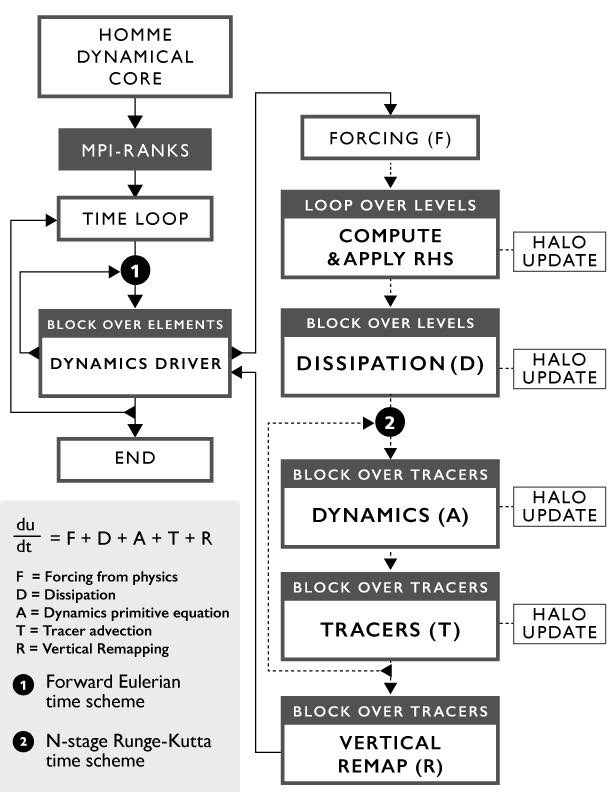
\includegraphics[width=12.0cm]{figures/HOMME-v00.png}
\end{center}
\caption{A plot of the memory usage of several different versions of CLM as function of processor count.  Elimination of both replicated data structures and global memory reduces memory usage for CLM at high resolution on 512 processors by a factor of 50.  }
\label{fig:clmmem}
\end{figure}


\subsubsection{Automatic kernel generation}

Using KGen is a simple one-step process which dramatically reduces the amount of time and resource that might be needed if kernel generation is done manually.  Figure 1 shows a workflow of using the tool.

Many scientific applications are large and complex. For example, CESM has more than 1.5 mil. SLOCs(source lines of code) and its own building system. Depending on configuration, it may takes more than an hour to complete compilation/execution. Instead, the size of generated kernel is generally between 1K to 100K SLOCs and it may take less than a minute to compile and run. Furthermore, a kernel does not have any dependencies to external library and could be easily built/run on multiple different machines. Therefore, once generated, kernel can be easily usable by collaborators.

Since a kernel is a just another software that can be compiled and run independently, its usage is not limited to a particular case. For example, There are several cases that KGen-generated kernel has been used successfully including:

Performance optimization: Several performance-critical parts of CESM were extracted using KGen and distributed to multiple performance engineers who independently optimized the generated kernels. Optimized kernels are collected and applied to CESM.

Validating Float-point calculation among different platforms: The same CESM simulation on two different system showed different simulation result. A “suspicious” part of code was extracted using KGen. After large number of trial-and-error on finding root cause of the difference, it is found that the root cause was a FMA(Fused-Multiply-Add) instruction. After switching-off FMA on one machine, the simulation result was the same to the other machine which does not have FMA.

Compiler bug report: A part of code that contains a compiler bug is extracted. A compiler bug is reported with the kernel so that the bug could be reproduced easily on compiler vendor site.

Porting a code on GPU: A part of radiation physics code is extracted and shared with an external research team for porting it on GPU.

Private benchmark for procurement: One of time consuming part of CESM is extracted and inserted in a benchmark suite for one of recent NCAR procurement.

\subsubsection{A kernel generation example}

KGen distribution package contains several examples. This section briefly steps through generating a kernel using one of the examples:“simple-region”.

First, please make sure that your system meets following prerequisites.
Linux OS
Python (higher or equal to 2.7 but less than 3.0)
Make build utility
Cpp C preprocessor
Strace system call tracer

Downloading KGen: run following Git command on your local directory.
>>>  git clone  https://github.com/NCAR/KGen.git

Or, you can directly download a compressed KGen release from “https://github.com/NCAR/KGen/releases”

Moving to an example directory: This example shows how to extract a region of Fortran code. Please read README to check if you need any modification to comply with your system.
>>> cd ./KGen/example/simple-region

Extracting a kernel: run make in the example directory. Please note that the make command actually invokes KGen command shown below.
>>> make

Above make command runs following KGen command.

\$KGEN/bin/kgen \
    --cmd-clean "cd src; make clean" \
    --cmd-build "cd src; make build" \
    --cmd-run "cd src; make run" \
    --timing repeat=100 \
    src/update\_mod.F90 

NOTE: \$KGEN is a path to KGen top directory.
NOTE: Actual KGen command in the example directory has more options.
NOTE: If paths on your system are aliased so that compilation path of application differs from where source codes reside, add %“--source alias=src_absolute_path:aliased_src_absolute_path” KGen option.
 
%First three options are to let KGen know how to clean/build/run the application. Next “--timing” option is to let KGen run a kernel region 100 times to increase accuracy of timing measurement as well as total execution time. The last line of argument specifies a path to a source file that contains KGen calllsite directives. User can specify any executable region of Fortran code as a kernel region by wrapping the region with “!$kgen begin_callsite <name>” and “!$kgen end_callsite [name]”. Please find KGen user’s guide for more information on the KGen directives.

Running a kernel: At this step, kernel files, state data files and Makefile are created in ��kernel�� subdirectory. KGen-generated Makefile in ��kernel�� folder makes it easy to build/run the kernel.
>>> cd kernel; make

Examining output from kernel execution: The extracted kernel is verified against state data generated from original software. Timing measurement is also displayed.

NOTE: NCAR has generated kernels from several weather/climate models. They can be downloaded from https://github.com/NCAR/kernelOptimization

